% Options for packages loaded elsewhere
\PassOptionsToPackage{unicode}{hyperref}
\PassOptionsToPackage{hyphens}{url}
%
\documentclass[
]{article}
\usepackage{amsmath,amssymb}
\usepackage{iftex}
\ifPDFTeX
  \usepackage[T1]{fontenc}
  \usepackage[utf8]{inputenc}
  \usepackage{textcomp} % provide euro and other symbols
\else % if luatex or xetex
  \usepackage{unicode-math} % this also loads fontspec
  \defaultfontfeatures{Scale=MatchLowercase}
  \defaultfontfeatures[\rmfamily]{Ligatures=TeX,Scale=1}
\fi
\usepackage{lmodern}
\ifPDFTeX\else
  % xetex/luatex font selection
\fi
% Use upquote if available, for straight quotes in verbatim environments
\IfFileExists{upquote.sty}{\usepackage{upquote}}{}
\IfFileExists{microtype.sty}{% use microtype if available
  \usepackage[]{microtype}
  \UseMicrotypeSet[protrusion]{basicmath} % disable protrusion for tt fonts
}{}
\makeatletter
\@ifundefined{KOMAClassName}{% if non-KOMA class
  \IfFileExists{parskip.sty}{%
    \usepackage{parskip}
  }{% else
    \setlength{\parindent}{0pt}
    \setlength{\parskip}{6pt plus 2pt minus 1pt}}
}{% if KOMA class
  \KOMAoptions{parskip=half}}
\makeatother
\usepackage{xcolor}
\usepackage[margin=1in]{geometry}
\usepackage{color}
\usepackage{fancyvrb}
\newcommand{\VerbBar}{|}
\newcommand{\VERB}{\Verb[commandchars=\\\{\}]}
\DefineVerbatimEnvironment{Highlighting}{Verbatim}{commandchars=\\\{\}}
% Add ',fontsize=\small' for more characters per line
\usepackage{framed}
\definecolor{shadecolor}{RGB}{248,248,248}
\newenvironment{Shaded}{\begin{snugshade}}{\end{snugshade}}
\newcommand{\AlertTok}[1]{\textcolor[rgb]{0.94,0.16,0.16}{#1}}
\newcommand{\AnnotationTok}[1]{\textcolor[rgb]{0.56,0.35,0.01}{\textbf{\textit{#1}}}}
\newcommand{\AttributeTok}[1]{\textcolor[rgb]{0.13,0.29,0.53}{#1}}
\newcommand{\BaseNTok}[1]{\textcolor[rgb]{0.00,0.00,0.81}{#1}}
\newcommand{\BuiltInTok}[1]{#1}
\newcommand{\CharTok}[1]{\textcolor[rgb]{0.31,0.60,0.02}{#1}}
\newcommand{\CommentTok}[1]{\textcolor[rgb]{0.56,0.35,0.01}{\textit{#1}}}
\newcommand{\CommentVarTok}[1]{\textcolor[rgb]{0.56,0.35,0.01}{\textbf{\textit{#1}}}}
\newcommand{\ConstantTok}[1]{\textcolor[rgb]{0.56,0.35,0.01}{#1}}
\newcommand{\ControlFlowTok}[1]{\textcolor[rgb]{0.13,0.29,0.53}{\textbf{#1}}}
\newcommand{\DataTypeTok}[1]{\textcolor[rgb]{0.13,0.29,0.53}{#1}}
\newcommand{\DecValTok}[1]{\textcolor[rgb]{0.00,0.00,0.81}{#1}}
\newcommand{\DocumentationTok}[1]{\textcolor[rgb]{0.56,0.35,0.01}{\textbf{\textit{#1}}}}
\newcommand{\ErrorTok}[1]{\textcolor[rgb]{0.64,0.00,0.00}{\textbf{#1}}}
\newcommand{\ExtensionTok}[1]{#1}
\newcommand{\FloatTok}[1]{\textcolor[rgb]{0.00,0.00,0.81}{#1}}
\newcommand{\FunctionTok}[1]{\textcolor[rgb]{0.13,0.29,0.53}{\textbf{#1}}}
\newcommand{\ImportTok}[1]{#1}
\newcommand{\InformationTok}[1]{\textcolor[rgb]{0.56,0.35,0.01}{\textbf{\textit{#1}}}}
\newcommand{\KeywordTok}[1]{\textcolor[rgb]{0.13,0.29,0.53}{\textbf{#1}}}
\newcommand{\NormalTok}[1]{#1}
\newcommand{\OperatorTok}[1]{\textcolor[rgb]{0.81,0.36,0.00}{\textbf{#1}}}
\newcommand{\OtherTok}[1]{\textcolor[rgb]{0.56,0.35,0.01}{#1}}
\newcommand{\PreprocessorTok}[1]{\textcolor[rgb]{0.56,0.35,0.01}{\textit{#1}}}
\newcommand{\RegionMarkerTok}[1]{#1}
\newcommand{\SpecialCharTok}[1]{\textcolor[rgb]{0.81,0.36,0.00}{\textbf{#1}}}
\newcommand{\SpecialStringTok}[1]{\textcolor[rgb]{0.31,0.60,0.02}{#1}}
\newcommand{\StringTok}[1]{\textcolor[rgb]{0.31,0.60,0.02}{#1}}
\newcommand{\VariableTok}[1]{\textcolor[rgb]{0.00,0.00,0.00}{#1}}
\newcommand{\VerbatimStringTok}[1]{\textcolor[rgb]{0.31,0.60,0.02}{#1}}
\newcommand{\WarningTok}[1]{\textcolor[rgb]{0.56,0.35,0.01}{\textbf{\textit{#1}}}}
\usepackage{graphicx}
\makeatletter
\def\maxwidth{\ifdim\Gin@nat@width>\linewidth\linewidth\else\Gin@nat@width\fi}
\def\maxheight{\ifdim\Gin@nat@height>\textheight\textheight\else\Gin@nat@height\fi}
\makeatother
% Scale images if necessary, so that they will not overflow the page
% margins by default, and it is still possible to overwrite the defaults
% using explicit options in \includegraphics[width, height, ...]{}
\setkeys{Gin}{width=\maxwidth,height=\maxheight,keepaspectratio}
% Set default figure placement to htbp
\makeatletter
\def\fps@figure{htbp}
\makeatother
\usepackage{soul}
\setlength{\emergencystretch}{3em} % prevent overfull lines
\providecommand{\tightlist}{%
  \setlength{\itemsep}{0pt}\setlength{\parskip}{0pt}}
\setcounter{secnumdepth}{-\maxdimen} % remove section numbering
\ifLuaTeX
  \usepackage{selnolig}  % disable illegal ligatures
\fi
\IfFileExists{bookmark.sty}{\usepackage{bookmark}}{\usepackage{hyperref}}
\IfFileExists{xurl.sty}{\usepackage{xurl}}{} % add URL line breaks if available
\urlstyle{same}
\hypersetup{
  pdftitle={2a-Getting Started for Mere Mortals},
  pdfauthor={DSC Chloe Farr},
  hidelinks,
  pdfcreator={LaTeX via pandoc}}

\title{2a-Getting Started for Mere Mortals}
\author{DSC Chloe Farr}
\date{2024-01-18}

\begin{document}
\maketitle

\hypertarget{getting-familiar-with-the-rstudio-interface}{%
\subsection{1. Getting familiar with the RStudio
Interface}\label{getting-familiar-with-the-rstudio-interface}}

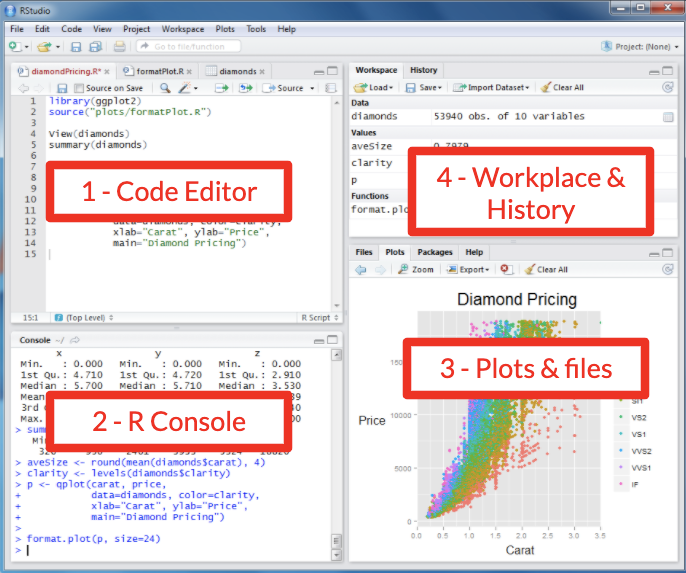
\includegraphics{images/rstudio-01.png} The RStudio interface is divided
into several key areas, each serving a specific purpose. - One of the
great features of RStudio is that you can customize the layout by
reorganizing these windows to suit your workflow.

\begin{verbatim}
*Hint:* You can rearrange these windows and tabs to fit your personal preference by dragging them around the workspace.<!--chloe make a video on rearranging windows and resetting--> When you rearrange the panes in RStudio on your computer, the layout stays as you set it across future sessions.
\end{verbatim}

\emph{Main components of the RStudio interface:}

\begin{enumerate}
\def\labelenumi{\arabic{enumi}.}
\item
  \emph{Code Editor:} This is where you write and edit your R scripts.

  \begin{itemize}
  \tightlist
  \item
    It features syntax highlighting, code completion, and other helpful
    tools to make coding easier.
  \end{itemize}
\item
  \emph{Console:} The console is where R code is executed.

  \begin{itemize}
  \item
    You can type commands directly into the console, and it displays
    outputs, messages, and errors.
  \item
    You might prefer to use the console for immediate execution, or
    testing of small code snippets or commands.
  \end{itemize}
\item
  \emph{Files/Plots/Packages/Help Pane:}
\end{enumerate}

\begin{itemize}
\item
  \emph{Files:} Browse, open, and manage files in your working
  directory.
\item
  \emph{Plots:} View graphical outputs from your R code, such as plots
  and graphs.
\item
  \emph{Packages:} Install, update, and load R packages.
\item
  \emph{Help:} Access R documentation and help files for:

  \begin{itemize}
  \tightlist
  \item
    functions and packages
  \item
    example code
  \item
    information about datasets built in to R
  \item
    information about other general R-related topics.
  \end{itemize}
\end{itemize}

\begin{enumerate}
\def\labelenumi{\arabic{enumi}.}
\setcounter{enumi}{3}
\tightlist
\item
  \emph{Environment/History Pane:}
\end{enumerate}

\begin{itemize}
\tightlist
\item
  \emph{Environment:} Shows your current workspace, including:

  \begin{itemize}
  \tightlist
  \item
    defined variables
  \item
    data frames
  \item
    function objects.
  \end{itemize}
\item
  \emph{History:} Records all the commands you've run in the current and
  previous sessions.
\end{itemize}

\ul{Task 1.1:} Open RStudio and get familiar with the interface by
identifying the 4 windows and switching between the tabs.

\begin{verbatim}
*Note:* This task is just for you to get comfortable. There is no solution for this task. <br>
\end{verbatim}

\hypertarget{working-in-the-code-editor}{%
\subsubsection{Working in the Code
Editor}\label{working-in-the-code-editor}}

Use the code editor if you want to develop more complex, reusable, and
maintainable code that can be saved and executed later. - We won't be
working in the code editor at this level. - It will be introduced at the
beginning of the Intermediate level workshop.

\hypertarget{working-in-the-console}{%
\subsubsection{Working in the Console}\label{working-in-the-console}}

The console is a lot like working in Terminal (mac) or Command
Prompt/PowerShell (PC). - Each new command line begins with the angle
bracket \texttt{\textgreater{}} also known as the `prompt' symbol.

You will type the commands into the Console after the most recent angle
bracket \texttt{\textgreater{}} also known as the `prompt' symbol. -
When you are ready to execute (`run') the command, type `enter' or
`return' key on your keyboard. - The output to the command will appear
below your command.

\emph{Things to be mindful of:}

\begin{itemize}
\item
  You cannot execute a command until the previous command has been
  completely executed.
\item
  If you don't see the prompt symbol, one of two things is happening:

  \begin{itemize}
  \item
    R is still processing your previous command, and you must wait for
    it to finish.
  \item
    You might instead see the plus \texttt{+} symbol, which indicates
    that you have entered an incomplete command.
  \end{itemize}
\item
  If you see the \texttt{+} symbol, you must enter the remainder of the
  command before entering a new one.
\item
  An error will occur if you write the \texttt{+} symbol into your
  command.
\item
  Sometimes the output can be extensive and show more information than
  you expected
\item
  E.g., when you load in a package (we will discuss packages more in
  Activity 3).
\end{itemize}

For all tasks in this workshop, enter your commands in the Console
(bottom left).

\ul{Task 1.2:} Try getting help! To do this, you'll run the
\texttt{help()} function. Try getting information on vectors.

Show Example

\begin{Shaded}
\begin{Highlighting}[]
\CommentTok{\#Get additional information about "vectors" (a data type), }
\FunctionTok{help}\NormalTok{(}\StringTok{"vector"}\NormalTok{) }\CommentTok{\# then type \textquotesingle{}enter\textquotesingle{} or \textquotesingle{}return\textquotesingle{}}
\end{Highlighting}
\end{Shaded}

\texttt{help("vector")} will provide you with information about the mean
function in RStudio. - The help information will be displayed in the
Console following your command.

Show/Hide Animation

\leavevmode\vadjust pre{\hypertarget{gif1}{}}%

\begin{verbatim}
*Note:* You can get help on related content by selecting the dropdown list at the top of the Help tab. <!--screenshot-->
\end{verbatim}

\begin{center}\rule{0.5\linewidth}{0.5pt}\end{center}

As you work through these activities, remember to save your workspace. -
Save your workspace by clicking on the top menu bar: - File - Save

\begin{center}\rule{0.5\linewidth}{0.5pt}\end{center}

\hypertarget{creating-and-manipulating-vectors-and-basic-variables}{%
\subsection{2. Creating and Manipulating Vectors and Basic
Variables}\label{creating-and-manipulating-vectors-and-basic-variables}}

Remember: Write all of your code in the \textbf{Console} tab.

\begin{verbatim}
*Note:* For the purposes of this workshop, 'variable' and 'data object' are used interchangeably.
\end{verbatim}

To create any data object: - the command will begin with the a name for
the new variable - followed by: - an assignment operator
\texttt{\textless{}-}, - and then the data or expression that defines
the content of the variable. - This can include direct values, function
calls, operations, or other variables.

\begin{verbatim}
variableName <- "word"
\end{verbatim}

\textbf{Definition - ``Function'':} A set of instructions defined to
perform a specific task.

\textbf{Definition - ``Function Call'':} The act of executing a function
with specific arguments, if required, to produce a result.

\hypertarget{variables-and-basic-data-types}{%
\subsubsection{2.1 Variables and Basic Data
Types}\label{variables-and-basic-data-types}}

Let's start by looking at types of variables.

\textbf{Definition - ``Basic Data Types'':} Types of data representing
the simplest forms of data.

\textbf{Basic Data Types}:

\begin{itemize}
\tightlist
\item
  \emph{Numeric}: Decimal or floating-point numbers (e.g., 4.5, -3.2).
\item
  \emph{Integer}: Whole numbers (e.g., 1, -5, 20).

  \begin{itemize}
  \tightlist
  \item
    In R, integers are often just treated as numeric unless explicitly
    specified.
  \end{itemize}
\item
  \emph{Character}: Text or strings (e.g., ``hello'', ``1234'').
\item
  \emph{Logical}: Boolean values, either TRUE or FALSE.
\item
  \emph{Factor}: Categorical data, or data as levels (e.g., ``low'',
  ``medium'', ``high'').
\end{itemize}

Here we'll look at basic operations with character variables.

\ul{Task 2.1.1:} Create a variable for a pig's first name. \textbar{}
\texttt{The\ first\ pig\textquotesingle{}s\ first\ name\ is\ \textquotesingle{}Bart\textquotesingle{}.}

Check Your Code

\begin{Shaded}
\begin{Highlighting}[]
\CommentTok{\#assign the first name \textquotesingle{}Bart\textquotesingle{} to the first pig (pig1)}
\NormalTok{pig1.first\_name }\OtherTok{\textless{}{-}} \StringTok{"Bart"}
\end{Highlighting}
\end{Shaded}

\ul{Task 2.1.2:} Create a variable for a Bart's last name. \textbar{}
\texttt{Bart\textquotesingle{}s\ last\ name\ is\ \textquotesingle{}Smith\textquotesingle{}.}

Show Code

\begin{Shaded}
\begin{Highlighting}[]
\CommentTok{\#assign the last name \textquotesingle{}Smith\textquotesingle{} to the first pig (pig1)}
\NormalTok{pig1.last\_name }\OtherTok{\textless{}{-}} \StringTok{"Smith"}
\end{Highlighting}
\end{Shaded}

\ul{Task 2.1.3:}

Create a variable that equals Bart's first and last name, then display
the full name in the console

Show Code

\begin{Shaded}
\begin{Highlighting}[]
\CommentTok{\#concatenate the first pig\textquotesingle{}s (pig1) first (\textquotesingle{}Bart\textquotesingle{}) and last name (\textquotesingle{}Smith\textquotesingle{})}
\NormalTok{pig1.full\_name }\OtherTok{\textless{}{-}} \FunctionTok{paste}\NormalTok{(pig1.first\_name, pig1.last\_name)}

\CommentTok{\#after pig1.full\_name has been created, print (display) Bart\textquotesingle{}s full name...}
\NormalTok{pig1.full\_name}
\end{Highlighting}
\end{Shaded}

\begin{verbatim}
## [1] "Bart Smith"
\end{verbatim}

\emph{Hint:} To combine two strings separated by a space, use the
\texttt{paste()} function.

Now we'll look at basic operations with \textbf{numeric and integer
variables}. First we'll create height information for Bart and find out
how much he's grown in height.

\ul{Task 2.1.4:} Create a variable for Bart's height as a piglet.
\textbar{} Bart's piglet height: 10

Show Code

\begin{Shaded}
\begin{Highlighting}[]
\CommentTok{\#Assign the value of Bart\textquotesingle{}s piglet height}
\NormalTok{pig1.heightA }\OtherTok{\textless{}{-}} \DecValTok{10}
\end{Highlighting}
\end{Shaded}

\ul{Task 2.1.5:} Create a variable for Bart's height now. \textbar{}
Bart's adult height: 22

Show Code

\begin{Shaded}
\begin{Highlighting}[]
\CommentTok{\#Assign the value of Bart\textquotesingle{}s current height}
\NormalTok{pig1.heightB }\OtherTok{\textless{}{-}} \DecValTok{22}
\end{Highlighting}
\end{Shaded}

\ul{Task 2.1.6:}

Now create a variable expressing the amount he's grown.

Show Code

\begin{Shaded}
\begin{Highlighting}[]
\CommentTok{\# Find the difference in height using the expression: \textquotesingle{}heightB {-} heightA\textquotesingle{} }
\CommentTok{\# using the subtraction operator. }
\NormalTok{pig1.heightGain }\OtherTok{\textless{}{-}}\NormalTok{ pig1.heightB }\SpecialCharTok{{-}}\NormalTok{ pig1.heightA}

\CommentTok{\#after pig1.heightGain has been created, print (display) the value of pig.heightGain...}

\NormalTok{pig1.heightGain}
\end{Highlighting}
\end{Shaded}

\begin{verbatim}
## [1] 12
\end{verbatim}

\emph{Hint:} ``Expressing'' indicates that the value will require an
expression, in this case, a mathematical operation.

Expand for information about numeric variables and functions

\texttt{pig1.heightA} is an `integer' data type (whole number)

\texttt{pig1.heightB} is a `numeric' data type (decmial number)

R can perform operations on different data types like getting the
difference of a value.

\begin{center}\rule{0.5\linewidth}{0.5pt}\end{center}

Reminder! Save your work

\begin{center}\rule{0.5\linewidth}{0.5pt}\end{center}

\begin{verbatim}
**Additional:** To display all objects you have created, execute the 'list' function in the console: `ls()`. \> *Note:* 'l' in 'ls' is the lowercase 'L'.

**Additional:** To remove data objects from your environment, execute the 'remove' function in the console: `rm()`.
\end{verbatim}

e.g., \texttt{rm(full\_name)}

\textbf{Time for logical or boolean values!}

We can denote if Bart is small or large with a boolean value.

\ul{Task 2.1.7:} \textbf{REWORK} default \emph{pig1.size} Create two
variables denoting Bart's general size. The Bart can either be `mini' or
`large'. Note that Bart is a large pig.

Show Code

\begin{Shaded}
\begin{Highlighting}[]
\NormalTok{pig1.mini }\OtherTok{\textless{}{-}} \ConstantTok{FALSE}

\NormalTok{pig1.large }\OtherTok{\textless{}{-}} \ConstantTok{TRUE}
\end{Highlighting}
\end{Shaded}

\emph{Hint:} Boolean values are either `TRUE' or `FALSE' (case
sensitive).

\textbf{DELETE} Expand to view the list of Environment Variables
(variables you have created in your environment)

If you have followed the code provided in the activities exactly, the
Variables list in your Environment tab should look the same as that in
the image below. If it doesn't match and you are unsure why, check with
the instructor. \textbf{no image}

\begin{verbatim}
Additional: Use the ls() function to see all of the variables in our environment so far.
\end{verbatim}

Show Code

\begin{Shaded}
\begin{Highlighting}[]
\FunctionTok{ls}\NormalTok{()}
\end{Highlighting}
\end{Shaded}

\begin{verbatim}
## [1] "pig1.first_name" "pig1.full_name"  "pig1.heightA"    "pig1.heightB"   
## [5] "pig1.heightGain" "pig1.large"      "pig1.last_name"  "pig1.mini"
\end{verbatim}

\hypertarget{vectors}{%
\subsubsection{2.2 Vectors}\label{vectors}}

A vector is a 1-dimensional list of items that are of the same data type
(all text, all whole numbers, etc.)

To create a vector object, you will use the \texttt{c()} function.

\begin{itemize}
\item
  The `c' stands for `combine' or `concatenate.'
\item
  It's used to create a vector by grouping individual values into a
  list-like structure.

  \begin{itemize}
  \item
    Think of it as placing items into a container where each item
    remains distinct and can be individually accessed.

    \begin{itemize}
    \tightlist
    \item
      For example, \texttt{vector1\ \textless{}-\ c(val1,\ val2)}
      creates a vector named `vector1' containing the elements `val1'
      and `val2' as separate items in a sequence, not as a single merged
      item.
    \end{itemize}
  \item
    A value in a vector can be accessed by using square brackets and its
    index (the value's place in the vector), where \textbf{1} is the
    first index.

    \begin{itemize}
    \tightlist
    \item
      \texttt{vector1{[}1{]}} will output: `val1'
    \end{itemize}
  \end{itemize}

  \emph{Note:} We will use the term `concatenate' later to merge
  strings. These have different meanings
\end{itemize}

As you might have seen if you tested the help() function by looking up
information on vectors, you will know that many functions and operations
in R are designed to work naturally with vectors.

\ul{Task 2.2.1:} Make a vector for the following weight values of
miniature goats. Name your variable `goat.weight'

\texttt{Goat\ weights:\ 13.3,\ 17.2,\ 14.8,\ 14.6,\ 12.4}

Show Code

\begin{Shaded}
\begin{Highlighting}[]
\CommentTok{\# The period between \textquotesingle{}goat\textquotesingle{} and \textquotesingle{}weight\textquotesingle{} has no special purpose. }
\CommentTok{\# It only shows the person reading the code that \textquotesingle{}weight\textquotesingle{} is information that pertains to \textquotesingle{}goat\textquotesingle{} }
\NormalTok{goat.weight }\OtherTok{\textless{}{-}} \FunctionTok{c}\NormalTok{(}\FloatTok{13.3}\NormalTok{, }\FloatTok{17.2}\NormalTok{, }\FloatTok{14.8}\NormalTok{, }\FloatTok{14.6}\NormalTok{, }\FloatTok{12.4}\NormalTok{)}
\end{Highlighting}
\end{Shaded}

The command you just ran has now appeared in your console (bottom left
window) - the goat.weight vector is now listed in the Environment tab
(top right window) under \ul{Values}.

If at any point you want to view the value of a variable or data
associated with a data object, simply enter the variable name and type
`enter' or `return' to execute.

\ul{Task 2.2.2:} Display (aka `print') the contents of the vector
containing the goat weights.

Show Code

\begin{Shaded}
\begin{Highlighting}[]
\NormalTok{goat.weight}
\end{Highlighting}
\end{Shaded}

\begin{verbatim}
## [1] 13.3 17.2 14.8 14.6 12.4
\end{verbatim}

\ul{Task 2.2.3:} Display the weight of the second goat in the vector.

Show Code

\begin{Shaded}
\begin{Highlighting}[]
\NormalTok{goat.weight[}\DecValTok{2}\NormalTok{]}
\end{Highlighting}
\end{Shaded}

\begin{verbatim}
## [1] 17.2
\end{verbatim}

\emph{Hint:} \emph{\texttt{data\_object\_name}}\texttt{{[}index{]}}

You have just worked with numeric vectors. Now let's move to string
vectors.

\ul{Task 2.2.4:} Make a vector for the following name values of
miniature goats. Name your variable `goat.name'

\texttt{Goat\ names:\ baby,\ pickles,\ cookie,\ sparkle,\ gabbie}

\begin{verbatim}
*Note:* Text values must be wrapped in quotations. You can use double or single quotes, but must be consistent - Good: "text" - Good: 'text' - Bad: 'text"
\end{verbatim}

Show Code

\begin{Shaded}
\begin{Highlighting}[]
\NormalTok{goat.name }\OtherTok{\textless{}{-}} \FunctionTok{c}\NormalTok{(}\StringTok{"baby"}\NormalTok{, }\StringTok{"pickes"}\NormalTok{, }\StringTok{"cookie"}\NormalTok{, }\StringTok{"sparkle"}\NormalTok{, }\StringTok{"gabbie"}\NormalTok{)}
\end{Highlighting}
\end{Shaded}

To get the length of a vector, we can use the length() function.

\ul{Task 2.2.5:} Print (display) the length of the vector of miniature
goat names.

\begin{verbatim}
*Note:* In a script (code editor), you often need to use the print() function explicitly to see the output, especially when running multiple lines of code or within functions. However, in the console, R automatically displays the output of expressions upon execution of the command.
\end{verbatim}

Show Code

\begin{Shaded}
\begin{Highlighting}[]
\FunctionTok{length}\NormalTok{(goat.name)}
\end{Highlighting}
\end{Shaded}

\begin{verbatim}
## [1] 5
\end{verbatim}

\hypertarget{additional-information-lists}{%
\paragraph{(Additional Information)
Lists}\label{additional-information-lists}}

A `list' can hold items of different types (even vectors), while items
in a `vector' must all be the same type.

To make a list, we'll use the \texttt{list()} function. \textgreater{}
\emph{Hint:} Remember that all items in a vector must be the same type,
but can be different types if in a list.

\emph{Additional:} If you want to create 2D lists, also known as a
table, you will create a matrix using the \texttt{matrix()} function. -
For more on matrices,
\href{https://www.w3schools.com/r/r_matrices.asp}{check me
out}\{:target=``\_blank''\}. - Instead of creating our own matrices, we
will be importing data later on.

\begin{center}\rule{0.5\linewidth}{0.5pt}\end{center}

Reminder! Save your work

\begin{center}\rule{0.5\linewidth}{0.5pt}\end{center}

\hypertarget{descriptive-statistics}{%
\subsection{3. Descriptive Statistics}\label{descriptive-statistics}}

Statistics is: - the science of collecting, analyzing, interpreting -
presenting data to uncover patterns and trends - making informed
decisions based on this data.

If you're unfamiliar with statistics, you can learn more about it from
the \href{https://www.w3schools.com/statistics/index.php}{w3school
Statistics Tutorial}\{:target=``\_blank''\}

In this section, we'll be focusing on - Basic statistical measures -
Presenting data in a histogram - More on presenting data will be covered
in
\href{https://uviclibraries.github.io/rstudio/ggplot2-data.html}{Activity
4-Data Visualization}\{:target=``\_blank''\} - Importing data

\hypertarget{basic-statistical-measures}{%
\subsubsection{3.1 Basic statistical
measures}\label{basic-statistical-measures}}

The function names for the following three statistical measures (mean,
median, standard deviation) are quite intutive. - It is just the name or
abbreviation of the measure, - where the argument is the object
containing the set of values we are analyzing. - Each function takes the
vector as its argument.

These three functions are designed for sets of numerical and decimal
values. If run on other types (text, boolean), result will be
\texttt{NA}.

For this task, we will use a new vector object containing weights for a
set of pigs.

\ul{Task 3.1.1:}

Create a vector object with the weights of a set of pigs. Name your
variable `pigs.weight'

\texttt{Weights\ of\ pigs:\ 22,\ 27,\ 19,\ 25,\ 12,\ 22,\ 18}

Show Code

\begin{Shaded}
\begin{Highlighting}[]
\NormalTok{pigs.weight }\OtherTok{\textless{}{-}} \FunctionTok{c}\NormalTok{(}\DecValTok{22}\NormalTok{, }\DecValTok{27}\NormalTok{, }\DecValTok{19}\NormalTok{, }\DecValTok{25}\NormalTok{, }\DecValTok{12}\NormalTok{, }\DecValTok{22}\NormalTok{, }\DecValTok{18}\NormalTok{)}
\end{Highlighting}
\end{Shaded}

\textbf{Mean:} the average value in a set.

This function calculates the sum of the in the set and divides the sum
by the number of items in the set. \texttt{mean()}

\ul{Task 3.1.2:} Write and execute a command that outputs the mean value
of the pigs' weights

Show Code

\begin{Shaded}
\begin{Highlighting}[]
\FunctionTok{mean}\NormalTok{(pigs.weight)}
\end{Highlighting}
\end{Shaded}

\begin{verbatim}
## [1] 20.71429
\end{verbatim}

This output is the average weight of all of the pigs

\textbf{Median:} The middle value in a sorted set (e.g.~lowest -
highest). \texttt{median()}

\ul{Task 3.1.3:}

Write and execute a command that outputs the median value of the pigs'
weights

Show Code

\begin{Shaded}
\begin{Highlighting}[]
\FunctionTok{median}\NormalTok{(pigs.weight)}
\end{Highlighting}
\end{Shaded}

\begin{verbatim}
## [1] 22
\end{verbatim}

The output tells you the weight of the pig that falls between the
lighter half and the heavier half of the pigs.

\textbf{Standard deviation:} Describes how spread out the data is.
\texttt{sd()}

\ul{Task 3.1.4:}

Write and execute a command that outputs the standard deviation of the
pigs' weights

Show Code

\begin{Shaded}
\begin{Highlighting}[]
\FunctionTok{sd}\NormalTok{(pigs.weight)}
\end{Highlighting}
\end{Shaded}

\begin{verbatim}
## [1] 4.956958
\end{verbatim}

The output tells you how much the weights of the pigs vary from the
average weight. - A small standard deviation means that most pigs'
weights are close to the average, indicating uniformity in size. - A
large standard deviation suggests a wide range of weights.

We can also execute a \textbf{`summary'} of our vector objects of the
pigs' weights to generate several descriptive statistics at the same
time.

\texttt{summary()}

\ul{Task 3.1.5:}

Display a summary of values pertaining to the pigs' weights

Show Code

\begin{Shaded}
\begin{Highlighting}[]
\FunctionTok{summary}\NormalTok{(pigs.weight)}
\end{Highlighting}
\end{Shaded}

\begin{verbatim}
##    Min. 1st Qu.  Median    Mean 3rd Qu.    Max. 
##   12.00   18.50   22.00   20.71   23.50   27.00
\end{verbatim}

\hypertarget{histogram-plot-for-pig-weights}{%
\subsubsection{3.2. Histogram Plot for Pig
Weights}\label{histogram-plot-for-pig-weights}}

\textbf{Histogram:} A graph used for understanding and analysing the
distribution of values in a vector.

\texttt{hist()}

A histogram illustrates: - Where data points tend to cluster - The
variability of data - The shape of variability

\ul{Task 3.2.1:}

Create a histogram for the pigs' weights.

Show Code and Histogram

\begin{Shaded}
\begin{Highlighting}[]
\FunctionTok{hist}\NormalTok{(pigs.weight)}
\end{Highlighting}
\end{Shaded}

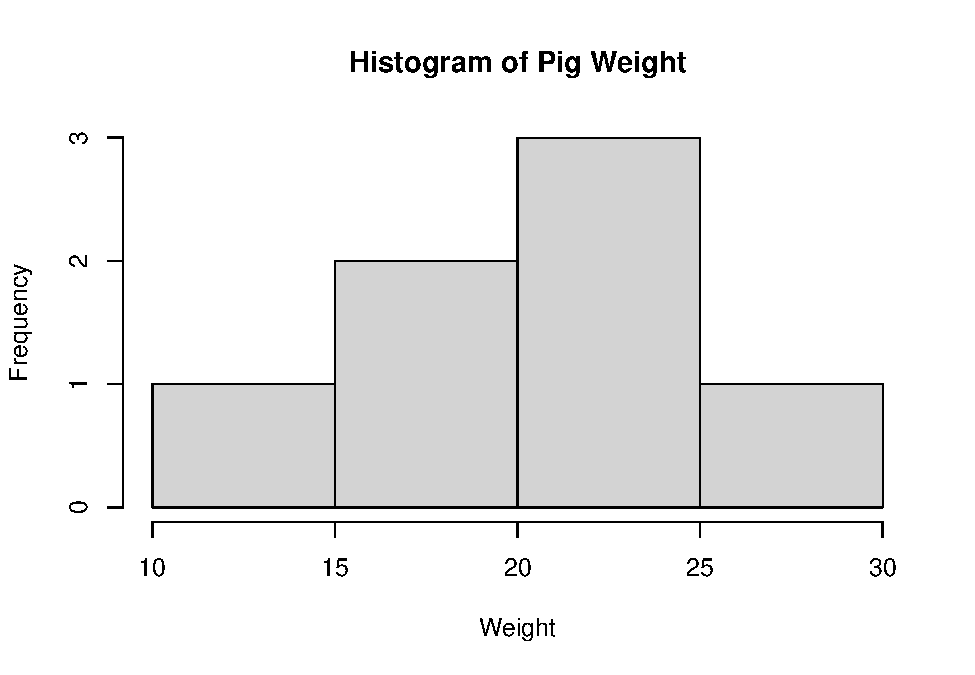
\includegraphics{basics0_files/figure-latex/unnamed-chunk-20-1.pdf}

\begin{Shaded}
\begin{Highlighting}[]
\CommentTok{\# The histogram will appear in the Plot tab.}
\end{Highlighting}
\end{Shaded}

The histogram will appear in the Plots tab (bottom right quadrant if you
haven't modified your RStudio layout).

We can also pass in additional parameters to control the way our plot
looks.

Some of the frequently used parameters are:

\begin{itemize}
\item
  \texttt{main} : The title of the plot

  \begin{itemize}
  \tightlist
  \item
    e.g., \texttt{main\ =\ "This\ is\ the\ Plot\ Title"}
  \end{itemize}
\item
  \texttt{xlab} : The x-axis label

  \begin{itemize}
  \tightlist
  \item
    e.g., \texttt{xlab\ =\ "The\ X\ Label"}
  \end{itemize}
\item
  \texttt{ylab} : The y-axis label

  \begin{itemize}
  \tightlist
  \item
    e.g., ylab = ``The Y Label''
  \end{itemize}
\end{itemize}

\ul{Task 3.2.2:}

Create a histogram for the pigs' weights, with axes labels.

\begin{itemize}
\tightlist
\item
  X-label: ``Weight''
\item
  Y-label: ``Frequency''

  \begin{itemize}
  \tightlist
  \item
    This is a default value.
  \item
    You don't have to specify it unless you would like a different
    label.
  \end{itemize}
\item
  Graph title: ``Histogram of Pigs' Weights''
\end{itemize}

\emph{Hint:} Remember, a parameter is information that goes in the
parenthesis of the function.

Single parameter: \texttt{function\_name(parameters)}

Multiple parameters: \texttt{function\_name(parameter1,\ parameter2)}

Show Code and Histogram

\begin{Shaded}
\begin{Highlighting}[]
\CommentTok{\# The first parameter is the name of the data (vector) object}
\CommentTok{\# \textquotesingle{}main\textquotesingle{} is the graph title }
\CommentTok{\# \textquotesingle{}xlab\textquotesingle{} is the label of the x{-}axis}
\CommentTok{\# label parameters can be in any order, but following the data object}

\FunctionTok{hist}\NormalTok{(pigs.weight,}\AttributeTok{main=}\StringTok{\textquotesingle{}Histogram of Pig Weight\textquotesingle{}}\NormalTok{,}\AttributeTok{xlab=}\StringTok{\textquotesingle{}Weight\textquotesingle{}}\NormalTok{)}
\end{Highlighting}
\end{Shaded}

\includegraphics{basics0_files/figure-latex/unnamed-chunk-21-1.pdf}

\begin{Shaded}
\begin{Highlighting}[]
\CommentTok{\# The histogram will appear in the Plot tab.}
\end{Highlighting}
\end{Shaded}

Additional: Use the ls() function to see all of the variables in our
environment so far.

Show Code

\begin{Shaded}
\begin{Highlighting}[]
\FunctionTok{ls}\NormalTok{()}
\end{Highlighting}
\end{Shaded}

\begin{verbatim}
##  [1] "goat.name"       "goat.weight"     "pig1.first_name" "pig1.full_name" 
##  [5] "pig1.heightA"    "pig1.heightB"    "pig1.heightGain" "pig1.large"     
##  [9] "pig1.last_name"  "pig1.mini"       "pigs.weight"
\end{verbatim}

\hypertarget{importing-data}{%
\subsection{4. Importing Data}\label{importing-data}}

So far, we've create our own objects by manually entering all of the
data in the console. In this section, we'll learn how to create objects
by importing (aka `reading') data (compiled outside of R) into R and
visualise it with a histogram.

\hypertarget{importing-excel-data-into-r}{%
\subsubsection{4.1 Importing Excel data into
R}\label{importing-excel-data-into-r}}

R can handle multiple file types:

\begin{itemize}
\tightlist
\item
  .csv (comma separated values)
\item
  excel (.xls, .xlsx)
\item
  .txt (and .tsv - tab separated values)
\item
  .json (used for nested data structures)

  \begin{itemize}
  \tightlist
  \item
    These would likely be arrays of more than 2 dimensions.
  \end{itemize}
\item
  SPSS (another specialized statistics software)
\item
  Data scraped from the web or via an API.
\end{itemize}

We can import data multiple ways. You'll import here through ``File'' in
the main menu. We'll look at other ways in the following activity pages.

\ul{Task 4.1.1}

Download and save \href{docs/income.xlsx}{this Excel spreadsheet of
Income data}\{:target=``\_blank''\} - \emph{Note: Please remember where
the income.xlsx file is saved (usually in a ``downloads'' or ``desktop''
folder).}

\ul{Task 4.1.3:} Import Import the dataset of Income data

\begin{itemize}
\item
  From the top menu bar, select\ldots{}

  \begin{itemize}
  \item
    File
  \item
    Import dataset
  \item
    From Excel
  \end{itemize}
\item
  In the `Import Excel Data' window select your file by:

  \begin{itemize}
  \item
    Entering the file path to the income.xlsx file you just downloaded.
  \item
    Selecting ``Browse'' on the right side of the path bar and locating
    it in the browser.
  \item
    Under `Import Options,' make sure `Name' is the same text as you
    wish for the variable to be named. Ours will be `income'.
  \item
    Click ``Import''
  \end{itemize}
\item
  ?? In \textbf{Yes} to install the ``\textbf{readxl}'' package.

  \emph{Note:} Don't worry about making a mistake importing this data.
  You can always remove it using the \texttt{rm()} function.
\end{itemize}

\begin{figure}
\centering
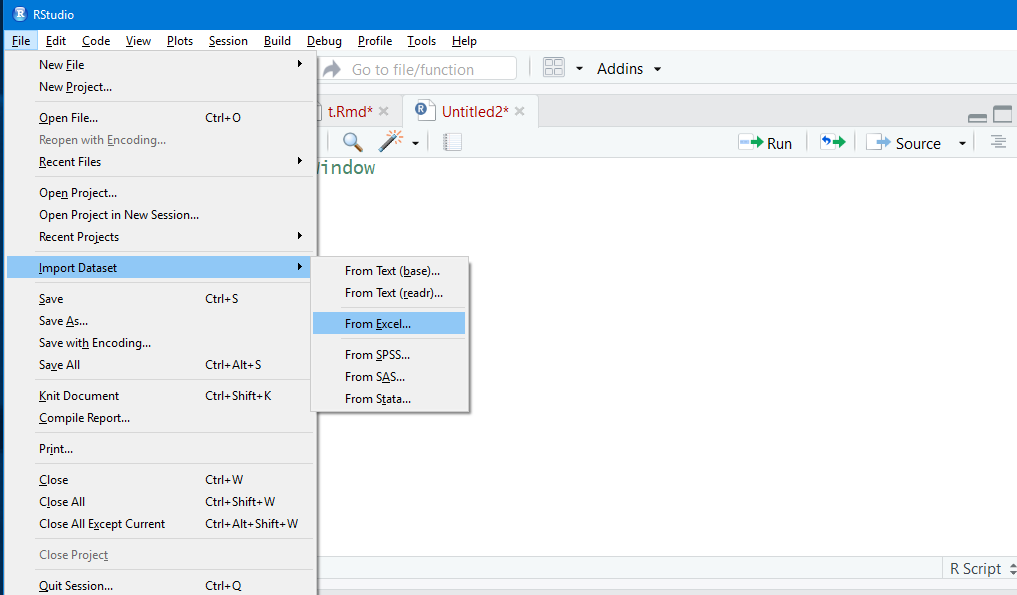
\includegraphics{images/rstudio-15.png}
\caption{Browse and import menu and buttons}
\end{figure}

\begin{figure}
\centering
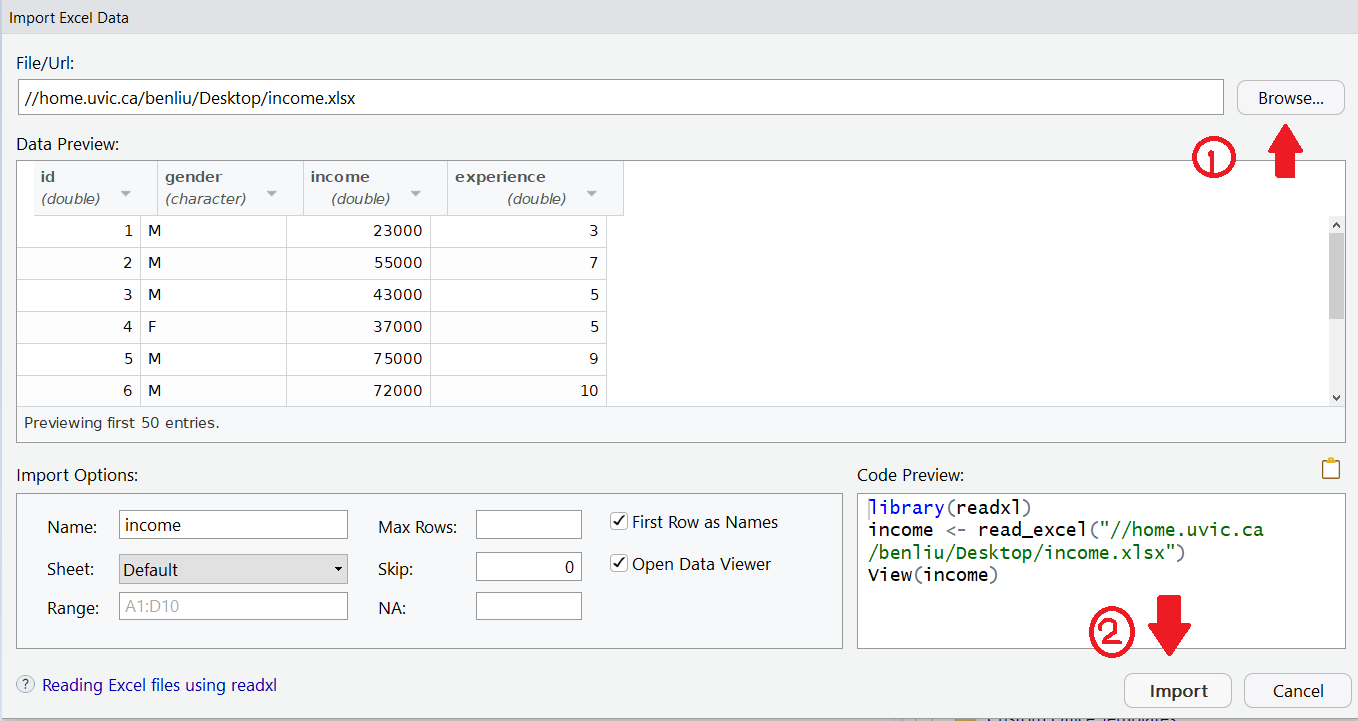
\includegraphics{images/rstudio-17.png}
\caption{Import excel data window}
\end{figure}

What you just imported is now stored as a `data frame' object whose name
is \texttt{income}.

\textbf{Definition - Data frame:} essentially a table. It is
2-dimensional object that can hold different types of data types.

\begin{verbatim}
*Additional:* Data frames contain information about a set of objects (e.g., cats).

-   The data frame will contain one or more columns and one or more rows.

-   One column contains related values (column 1 = age, column 2 = eye color).
\end{verbatim}

\begin{itemize}
\item
  Because the column contains the same type of information, it is
  equivalent to a vector. I.e., the `eye color' column will contain
  characters, not numbers.
\item
  One row denotes one object from the set. In a data frame of
  information about a set of cats, each row is information about one
  specific cats.

  A row can contain many different bits of information, like age
  (numerical), eye color (character), breed (character), whether or not
  it's spayed/neutered (boolean). Because rows may contain values of
  different types, one row would most likely not be a vector. It would
  likely be a list, which can contain values of different types.
\end{itemize}

To see the data in our data frame, simply enter the name of the data
frame in the console and type `enter' or `return'.

Show code

\begin{Shaded}
\begin{Highlighting}[]
\NormalTok{income}
\end{Highlighting}
\end{Shaded}

The following will be the output:

\begin{verbatim}
## # A tibble: 10 x 4
##       id gender income experience
##    <dbl> <chr>   <dbl>      <dbl>
##  1     1 M       23000          3
##  2     2 M       55000          7
##  3     3 M       43000          5
##  4     4 F       37000          5
##  5     5 M       75000          9
##  6     6 M       72000         10
##  7     7 F      121000         13
##  8     8 F       27000          1
##  9     9 F       57000          8
## 10    10 F       91000         10
\end{verbatim}

\begin{verbatim}
*Note:* We will explore other ways to view and preview content of our data frames in Activity 3.

*Note:* `<char>` stands for "character" data type and `<dbl>` stands for "double-precision floating point numbers data" type. <br>
\end{verbatim}

We can see now that our data frame \texttt{income} contains 10 objects
(rows), and 4 variables (columns) - It can be inferred that this data
relates to 10 people - The values with each person are: - id (in lieu of
a name) (dbl) - gender (char) - income (dbl) - experience (dbl)

Task 4.1.3:

Display a summary of statistics for the \texttt{income} data.

Show Code

\begin{Shaded}
\begin{Highlighting}[]
\FunctionTok{summary}\NormalTok{(income)}
\end{Highlighting}
\end{Shaded}

\begin{verbatim}
##        id           gender              income         experience   
##  Min.   : 1.00   Length:10          Min.   : 23000   Min.   : 1.00  
##  1st Qu.: 3.25   Class :character   1st Qu.: 38500   1st Qu.: 5.00  
##  Median : 5.50   Mode  :character   Median : 56000   Median : 7.50  
##  Mean   : 5.50                      Mean   : 60100   Mean   : 7.10  
##  3rd Qu.: 7.75                      3rd Qu.: 74250   3rd Qu.: 9.75  
##  Max.   :10.00                      Max.   :121000   Max.   :13.00
\end{verbatim}

\hypertarget{visualize-income-with-a-histogram-plot}{%
\subsubsection{4.2 Visualize Income with a Histogram
plot}\label{visualize-income-with-a-histogram-plot}}

In 3.2 we made a histogram to visualize the distribution of the pig
weights. Remember that the parameter that the histogram function takes
is a vector.

To extract a vector (column) from our data frame, we will pass in
\texttt{\_dataframeName\_\$\_columnName\_}, where the name of our data
is separated by the name identifying a single set of values within that
data frame.

Task 4.2.1

Display the vector of data relating to `experience' in a histogram. -
X-label: `Experience' - Title: `Histogram of Experience'

Show Code

\begin{Shaded}
\begin{Highlighting}[]
\CommentTok{\#Remember, the generated histogram will appear in the Plot tab.}
\FunctionTok{hist}\NormalTok{(income}\SpecialCharTok{$}\NormalTok{experience, }\AttributeTok{main=}\StringTok{\textquotesingle{}Histogram of Experience\textquotesingle{}}\NormalTok{,}\AttributeTok{xlab=}\StringTok{\textquotesingle{}Experience\textquotesingle{}}\NormalTok{)}
\end{Highlighting}
\end{Shaded}

The following will be the output:

\includegraphics{basics0_files/figure-latex/unnamed-chunk-27-1.pdf}

We can see in the histogram that there are 7 intervals with equally
spaced breaks. In this case, the height of a cell is equal to the number
of observations falling in that cell. - Why are there 7 intervals? R
automatically chooses the number of intervals for you.

\emph{Additional:} If you preferred having 4 intervals (i.e., `bins'),
use can set that using the
\texttt{breaks=\textquotesingle{}\textquotesingle{}} parameter.

Show code for custom number of intervals

\begin{Shaded}
\begin{Highlighting}[]
\CommentTok{\#breaks is equal to the number of intervals}
\FunctionTok{hist}\NormalTok{(income}\SpecialCharTok{$}\NormalTok{experience, }\AttributeTok{main=}\StringTok{\textquotesingle{}Histogram of Experience\textquotesingle{}}\NormalTok{,}\AttributeTok{xlab=}\StringTok{\textquotesingle{}Experience\textquotesingle{}}\NormalTok{, }\AttributeTok{breaks=}\DecValTok{4}\NormalTok{)}
\end{Highlighting}
\end{Shaded}

\includegraphics{basics0_files/figure-latex/unnamed-chunk-28-1.pdf}

\end{document}
